\chapter{Contribution \& Discussion}
In this chapter we propose our data warehouse and visualization system for medical data that aims to manage the uncommon data from the various sources using a conventional common language between the different health actors.




\section{Work Objectives}
The aim of this work is to propose a data warehouse system that organizes data coming from different sources by producing a common language. We are interested in the step between Rendering and Data image in the pipeline process(\ref{fig:infovispipeline}). After reviewing and analyzing similar proposed works, we created our own visualization system for medical data in a conventional common language.





\section{Literature \& Related works review}
We present in this section architecture for healthcare data warehouses and solutions that attempt to integrate infoVis into medical data and medical structures which could be used by executive managers, doctors, physicians and other health professionals to support the healthcare process.  Medical data existing today in multiple sources with different formats makes it necessary to have certain data integration techniques. A healthcare data warehouse is therefore needed to integrate the different data sources into a central data repository and analyze this data.

\begin{itemize}
  \renewcommand{\labelitemi}{$\bullet$}
  \item \textbf{\textit{A Healthcare Data Warehouse for Cancer Diseases:}} Dr.Osama E.Sheta and Ahmed Nour Eldeen discussed in their paper\cite{shetaBuildingHealthCare2012} the implementation of a healthcare data warehouse for cancer diseases, they proposed  two stages approach for the building cancer data warehouse: 
  
  \begin{enumerate}
    \item \textit{Business Analysis:} Consist of business process analysis and business requirement analysis (Figure\ref{fig:cancerDiagrame}).
    \begin{figure}[h!]
      \center
      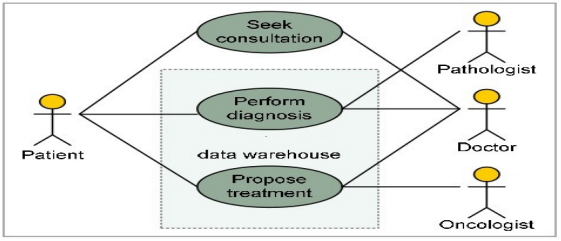
\includegraphics[width=0.75\textwidth]{images/chapter3/cancerDiagrame.PNG}
      \caption{Cancer data warehouse use case diagram.}
      \label{fig:cancerDiagrame}
    \end{figure}
    \item \textit{Architecture Design:} Data is imported from several sources and transformed within a staging area before it is integrated and stored in the production data warehouse for further analysis (Figure\ref{fig:cancersystem}).
     \begin{figure}[h!]
      \center
      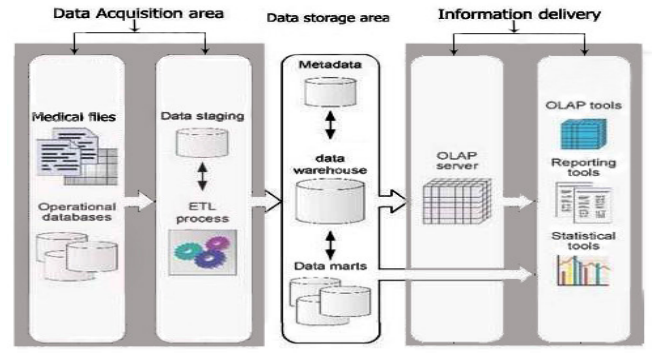
\includegraphics[width=0.75\textwidth]{images/chapter3/cancersystem.PNG}
      \caption{Cancer data warehouse Architecture Taken from the source.}
      \label{fig:cancersystem}
    \end{figure}
    \end{enumerate}
    
    \item \textbf{\textit{Data Warehouse Framework in Pharmaceutical Sector:}} In this paper\cite{abd2019proposed} authors proposed a data warehouse framework to enhance decisions of distribution systems in pharmaceutical companies to decrease the medicine industry cost and increase productivity. The framework can be described in four phases shown in (Figure \ref{fig:pharmacysystem}). Phase one consists of a data preparation, a phase which has four steps (data collection, building DBs, DWH and data cleaning). Phase two consists of training the data which is applying time series to three types of Neural Networks techniques (levenberg marquardt, Bayesian regularized, and Scaled conjugate gradient). Phase three is testing the performance based on mean square error (MSE). Phase four consists of evaluating the performance of the best prediction model.
    \begin{figure}[h!]
      \center
      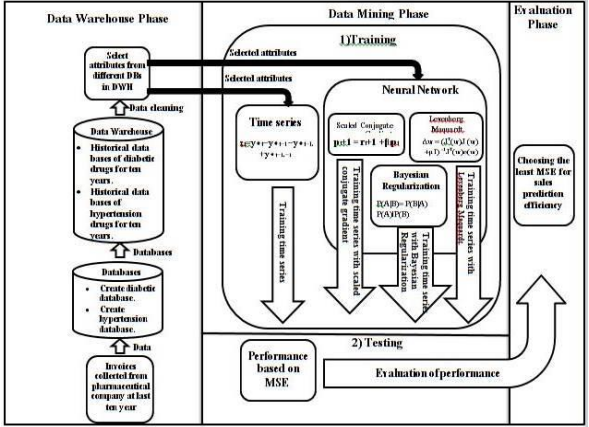
\includegraphics[width=0.75\textwidth]{images/chapter3/pharmacysystem.PNG}
      \caption{The Proposed Framework of Sales Prediction.}
      \label{fig:pharmacysystem}
    \end{figure}
    
    \item \textbf{\textit{Big Bata Warehouse Based On Hadoop Architecture:}} In this paper\cite{sebaa2018medical} entitled “Medical Big Data Warehouse: Architecture and System Design, a Case Study: Improving Healthcare Resources Distribution” authors proposed a system architecture and a conceptual data model for a MBDW (Medical Big Data Warehouse), and then offer a solution to overcome both the growing of fact table size and the lack of primary and foreign keys in the framework Apache Hive required in the conceptual data model. This solution is based on nested partitioning according to the dimension tables keys, then  applying their solution to implement a MBDW to improve medical resources distribution for the health sector in the Bejaia region (in Algeria). 
    \newpage
    The overall architecture is depicted in (Figure \ref{fig:bigdatarelated}). It is a scalable, reliable, and distributed architecture to extract, store, analyze, and visualize healthcare data extracted from various resources HIS (Hospitals Information systems).
    \begin{figure}[h!]
      \center
      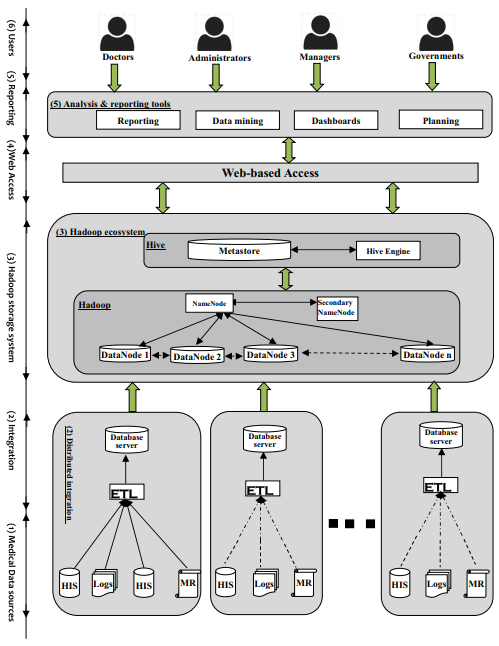
\includegraphics[width=0.50\textwidth]{images/chapter3/relatedworkHadoop.PNG}
      \caption{Hadoop-based system architecture of medical big data warehousing.}
      \label{fig:bigdatarelated}
    \end{figure}
\end{itemize}


\section{Proposed Solution}
As mentioned in the project description, the presence of a visualization presentation in the medical sector is necessary. The proposed solution was to create a system that organizes the data and structures it, we used for that the eXtensible Markup Language (XML).
We mainly focused on the "Rendering" step in the visualization pipeline(\ref{fig:infovispipeline}), and we worked on the medical data that are mentioned in the Table\ref{tab:sourceTable}.
\newpage
\subsection{Why XML?}
The rise of XML (eXtensible Markup Language) in patient care has been driven by the needs for communication among health professionals and between healthcare organizations such as hospitals and health insurance companies.The main advantage of XML is its flexibility, as it allows creators to describe any content easily by generating their own tags\cite{thuy2012s}. Some of XML’s features are\cite{achard2001xml}:
\begin{itemize}
\renewcommand{\labelitemi}{$\bullet$}
\item The XML and DTD files are human readable and thus can be easily edited by people with only a few computer skills. Updating a data model is, therefore, straightforward (at least from a technical point of view).
\item XML is Internet-oriented and has very rich capabilities for linking data; this can be used for interconnecting databases.
\item XML provides an open framework for defining standard specifications. This is an important point because medical informatics clearly lacks standardization. For example, querying on multiple molecular biology databases could be greatly facilitated if each database would offer an XML view of their content.
\end{itemize}
On the other hand, XML has some weaknesses:
\begin{itemize}
\renewcommand{\labelitemi}{$\bullet$}
\item The overhead of a text based format in data parsing, storage and transmission needs to be evaluated before adopting XML as a general solution. However, a text format means that the source code can be read and edited with any text editor.
\item It is not clear whether XML satisfactorily addresses the problems of technological scalability. Indeed if XML data are stored in flat files, queries on XML files will not scale because XML in itself does not provide scalable facilities such as indexing or data clustering. This means that parsing should be done on the fly which leads to poor performances. One solution could be to have query optimizations done externally for example using a DataBase Management System (DBMS).
\end{itemize}
\newpage
At this point the question to be answered is whether the pros prevail over the cons, for this reason Frederic Achard and al\cite{achard2001xml}  have provided a comparison between XML and some of the most popular solutions that are used for the management and exchange of bioinformatics data summarized in the (Table\ref{tab:xmlcomparaison}), each one is rated with one to four stars for different criteria: the higher the number of stars, the better the solution with regard to the criteria.
\begin{table}[h!]
    \centering
    \begin{tabular}{|m{0.20\linewidth}|m{0.10\linewidth}|m{0.10\linewidth}|m{0.10\linewidth}|m{0.11\linewidth}|m{0.10\linewidth}|m{0.10\linewidth}|}
        \hline

        \textbf{Criteria}                      & \textbf{XML}        & \textbf{{\small Field/ value} }        & \textbf{{\small \gls{asn}}}    & \textbf{{\small \gls{cobra}}} &\textbf{{\small \gls{java}}}      & \textbf{{\small \gls{oodbms}}}      \\

        \hline
        Model expressiveness 	& **	& *		& *** & *** & *** & ****     \\
        
        \hline
        Constraints	    & **	& *	& *    & **   & ***   & ****       \\
        
        \hline
        Self-descriptive    & yes	& no	& yes    & yes   &  yes  &  yes      \\
        
        \hline
        Query language	 & soon 	& no	& no    & soon    & no   &  yes \\
        
        \hline
        Flexibility	 & ****	& *	& ***    &  ***  & ***   & ****  \\
        
        \hline
        Simplicity 	 & ****	& ****	& ***    & *   & **   & **  \\
        
        \hline
        Scalability 	 & **	& *	& **   & ***   & ***   & ****  \\
        
        \hline
        Interoperability 	 & ****	& *	&  **  & ****   & ****   & ***  \\
                
        \hline
    \end{tabular} 

    \caption{Summary of comparison of different alternatives to XML.}
    \label{tab:xmlcomparaison}
\end{table}
\bigbreak
They conclude that the use of XML as an intermediate medium would be really efficient only if all databases share common or very similar DTDs. Whatever language is used, it is always difficult to find an agreement on a common semantics, and when one is found, it is often revised. However, XML would be an excellent candidate for this role because of its flexibility.



\subsection{Architecture}



We focused on extracting the following type of data (each head represents an XML node):
\begin{itemize}
\renewcommand{\labelitemi}{$\bullet$}
\item \textbf{Patient:} That presents the administrative information about the patient x, including his full name, gender, date of birth, address. 
\item \textbf{Drug:} Presents the list of drugs in the patient’s  prescription, it includes: the drug’s name, its dosage, strength usually mentioned by the doctor, the quantity, and its type(liquid or table).
\item \textbf{Diagnosis:} Includes the doctor's name, the diseases name, and the observations taken by the medical actor in charge, it also contains the name of the prescribed medications and the date of diagnosis. 
\item \textbf{LabResults:} It presents the medical biology results that includes the analysis’s name,the patient rate saved, the gender and the age for the comparison (a predefined high/low rate is defined corresponding to each analysis), attached with the laborator name.
\item \textbf{ImagesData:} Present the data of the image obtained by the patient, it includes the image name and the image itself, the day it was taken, and the patient's national ID number.
\end{itemize}
\begin{figure}[h!]
  \center
  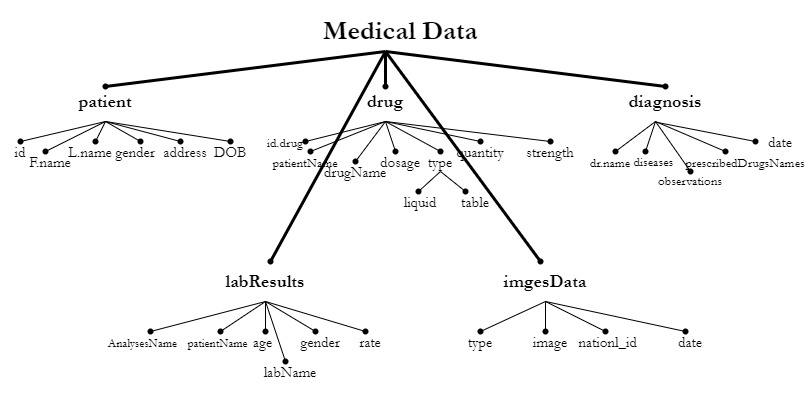
\includegraphics[width=0.99\textwidth]{images/chapter3/tree.jpg}
  \caption{The corresponding tree of XML schema.}
  \label{fig:xmlschema}
\end{figure}
\newpage
\subsection{Data Integration \& Processing}

Our main objective was to create a visualization system for that: we collected medical data from different sources that represent various medical actors, and we process them following the visualization process mentioned before (\ref{fig:infovispipeline}), we used Talend open studio (\ref{sec:talend}) to handle this step.

The resulting data will be used as a source to feed all the components of the digital marketing reporting applications that are built in many visualization tools.
\begin{figure}[h!]
  \center
  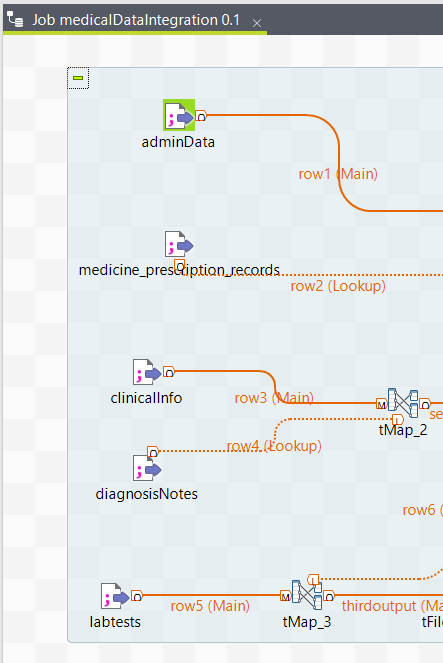
\includegraphics[width=0.30\textwidth]{images/chapter3/jobInputs.PNG}
  \caption{Input data.}
  \label{fig:jobinputes}
\end{figure}
\begin{figure}[h!]
  \center
  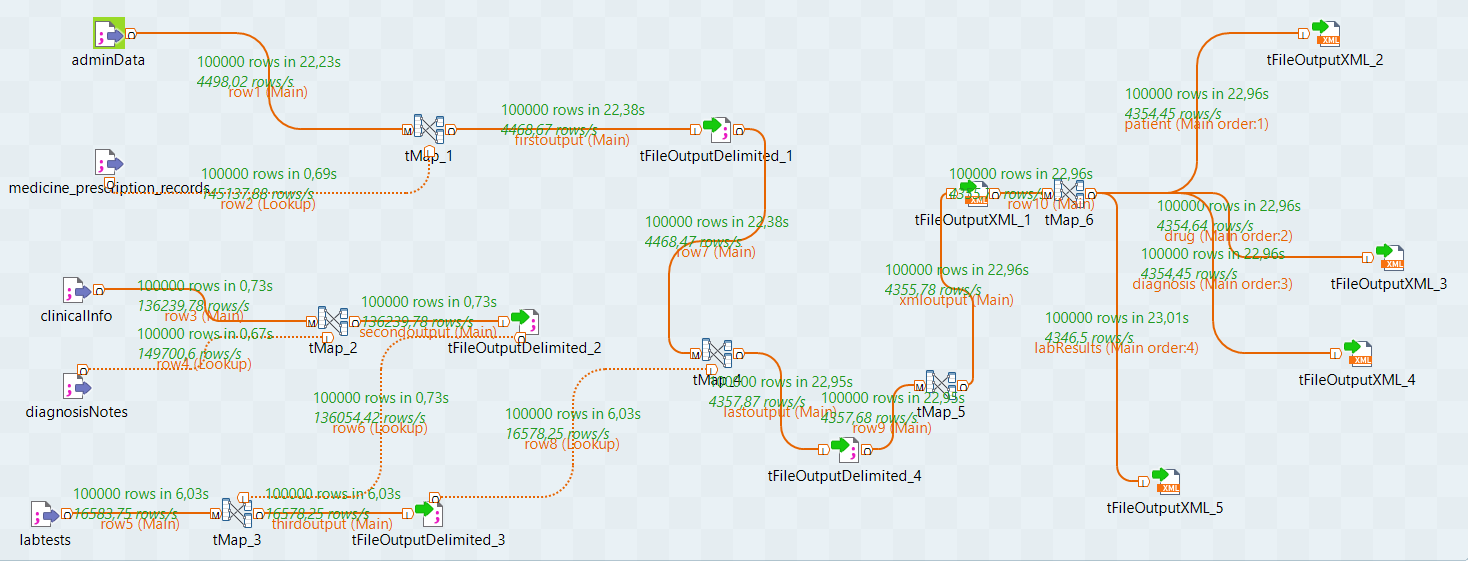
\includegraphics[width=0.80\textwidth]{images/chapter3/jobresult.PNG}
  \caption{Talend job execution.}
  \label{fig:jobtalend}
\end{figure}